\chapter{Implementation of k-Means in HyPer}\label{chapter:implementation}

In this chapter we present the implementation of the k-Means algorithm as a HyPer operator. First we discuss the general implementation of operators in HyPer, the used programming model and the LLVM code generation. Then, the constraints and requirements of the k-Means implementation are introduced. Next, the implementation details are depicted including data materialization, a C++ driven version and an LLVM driven version. Additionally to the random initialization strategy the k-Means++ initialization strategy is implemented as described in Section~\ref{section:kmeans_init}. Finally, a parallel realization of the k-Means operator is discussed.


\section{HyPer Operator Fundamentals}\label{section:operator}

In this section we discuss the general implementation of operators in HyPer and the involved code generation. With this programming model in mind we can afterwards show how the k-Means operator is implemented in HyPer. The argumentation and results of this section are based on~\parencite{neumann} and~\parencite{neumann+leis}.

\subsection{The Consume Produce Programming Model}
As all data resides in memory, main memory databases' query performance is much more dependent on the CPU cost of the query processing than on I/O cost as in traditional systems. Therefore, query processing has to be reinvented to achieve optimal performance.
Before a query is executed, most database systems translate a query into an algebraic expression and start evaluating and executing this algebraic plan. Traditionally, this is done using the iterator model~\parencite{iterator}: Each physical operator produces a tuple stream and iterates to the next tuple by calling the~\texttt{next} function of the operator. The iterator model works well for I/O dominated, traditional databases, where CPU consumption is not a limiting factor. However, for main memory databases, this is not perfect: First,~\texttt{next} is called many times, once for every single tuple for each intermediate and final result. This~\texttt{next} call is usually a virtual call or a call via function pointer which makes it more expensive than a regular call and reduces branch prediction of modern CPUs. Moreover, the iterator model results often in poor code locality and complex bookkeeping. This can be seen from the functionality of the table scan operator: As tuples are generated one after the other, the operator has to remember where in the compressed stream the current tuple was and has to jump back when asked for the next one. 
\\
In order to resolve these issues, Neumann~\parencite{neumann} proposes a new query compilation strategy for main memory databases: Instead of the operator centric approach of the iterator model, processing is data centric. Therefore data can be kept in the CPU registers as long as possible, while the boundaries between the operators get more and more blurred. That means that each code fragment performs all actions on the given data, until the result has to be materialized, i.e. data is taken out of the registers. A code structure like this generates almost optimal assembly code, since all the relevant instructions for the given data are generated, and therefore the data can be kept in the CPU registers.
\\
HyPer uses a simple programming model for its operators in order to make  compilation as efficient as possible, while writing code remains understandable and maintainable for the developer: Each operator implements two functions, a \texttt{consume} and a \texttt{produce} function. The \texttt{produce} function computes the result tuples of an operator, which are then pushed to the next operator by calling its \texttt{consume} function. The next operator works the same way, after getting data in by a \texttt{consume} call of the predecessor, it produces result tuples by calling its own \texttt{produce} function. To wrap it up, each operator gets its own \texttt{consume} function called by its predecessor, calls its own \texttt{produce} function to compute the results and calls then the \texttt{consume} function of its successor. This process is shown in the sequence diagram in~\autoref{fig:consume_produce_sd}.


\begin{figure}[htsb]
  \centerline{
      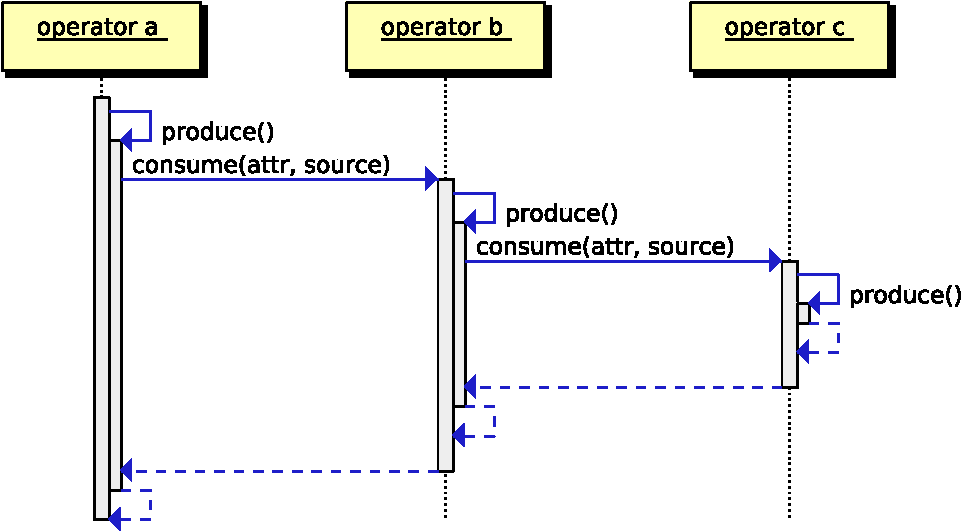
\includegraphics[scale=0.7]{figures/consume_produce}
  }
  \caption[Consume Produce Sequence Diagram]{Consume Produce Sequence Diagram.}\label{fig:consume_produce_sd}
\end{figure}


Therefore, this programming model pushes data towards the next operator, instead of pulling the data. This results in a much better code and data locality. Tuples are pushed from one operator to the next, therefore operators benefit from keeping the data in the CPU registers, which allows very cheap and efficient computation. Only for materializing data memory has to be accessed. Additionally, small code fragments are used to handle large amounts of data in tight loops leading to good code locality and therefore high performance.
\\
These aspects make the execution of operators very fast. Unfortunately, not all operators can be implemented in a way that one tuple gets fully processed before the next one is loaded into the CPU registers. Instead, tuples have to be taken out of the registers and are materialized in main memory for some operators. Those operators break the operator pipeline, therefore we call them~\emph{pipeline breakers}. If an operator materializes all incoming tuples before continuing processing, we call it a~\emph{full pipeline breaker}. An example is a join operator: One side of the two join relations has to be materialized in main memory,  while the other relation is scanned and probed against the materialized data for finding join partners. As the join operator materializes one relation it is a~\emph{pipeline breaker}.
\\
Finally, it is important to note that the \texttt{consume produce} model is just an abstraction layer for the programmer. This abstraction layer is used by the code generation to compile assembly code - within the generated assembly code there is no \texttt{consume produce} present anymore.

\subsection{LLVM Code Compilation}

In this section we discuss the query compilation in greater detail. As in traditional systems, queries are compiled by parsing the query, translating it into algebra and optimizing it. In contrast to a traditional system, the physical algebra is not directly executed, but compiled by the code generation into an imperative program. For generating this imperative program the previously described ~\texttt{consume produce} model is used.
\\
Taking advantage of the structure of the~\texttt{consume produce} model, queries are compiled into native machine code using the LLVM compiler framework~\parencite{LLVM}. LLVM can generate portable assembler code which can be executed directly using an optimizing JIT compiler. With LLVM HyPer uses a very robust assembly code generation, e.g. pitfalls like register allocation are hidden by LLVM. Therefore the assembly code generation is very convenient compared to other compiler frameworks. Furthermore, only the LLVM JIT compiler translates the code into machine dependent code, leading to portable code across computer architectures. Since the LLVM assembler is strongly typed, many bugs can be caught in advance, in contrast to a textual C++ code generation. Furthermore, LLVM produces highly optimized, extremely fast machine code and outperforms in some cases even hand-written code as the assembly language allows code optimization, hardware improvements and other tricks, that are hard to do in a language like C++. All this requires usually only a few milliseconds of compilation time, which is a crucial criterion for database operators with a strong focus on performance.
\\
Additionally, LLVM code is perfectly able to interact with C++, the main language of the HyPer database. Even though LLVM code is robust and convenient to write compared to common assembler code, it is still more painful than writing code in a high-level language such as C++. An interaction of the two languages allows us to implement complex structures in C++ and to reuse existing database logic such as index structures. 
\\
Therefore algorithms can be written in C++ and connected together by LLVM code, where the C++ code is pre-compiled and the LLVM code is compiled at runtime dynamically. An example is the Sort operator: The \texttt{compare} function, comparing two tuples by the rules of a sort query is dynamically generated in LLVM code, depending on the schema of the database. As actual sort function, the built-in C++ \texttt{sort} can be used. This is a great example of the mixed execution model using C++ and LLVM code in one operator.
\\
However, even though C++ and LLVM can both be used implementing an operator, LLVM code is dominant and C++ code should be seen as convenience. For performance reasons it is important that the code executed for most of the tuples is generated code, even though calling C++ from time to time is acceptable. As already mentioned, staying in LLVM allows us to keep the data in the CPU registers and is therefore the preferable way of executing a query. Calling an external function spills all registers to memory, which can be a bottleneck when doing this for all tuples in a big data set.
\\
In conclusion, we have presented the HyPer~\texttt{consume produce} programming model which allows operators to push data towards the next operator in an efficient manner. Furthermore, the LLVM compiler framework with its benefits is introduced used for code generation and interacting with C++ code at runtime. 
This cooperation of LLVM and C++ code regarding programmer friendliness and execution time is one of the dominant patterns in Section~\ref{section:serial_implementation}, where two alternative implementations of the k-Means operator are presented and discussed. 


\section{Requirements and Constraints}
Before discussing the technical implementation details of the k-Means operator, we introduce the requirements and constraints. Obviously, the k-Means algorithm must be implemented as a HyPer operator. That means, the \texttt{consume produce} programming model and the code generation with C++ and LLVM have to be used. The advantage of implementing k-Means as an operator is that it can be used in combination with existing SQL operators, useful for data mining as well, such as grouping and aggregation.
\\
Regarding the functional aspects, the operator must be able to be executed in serial and in parallel, to make use of the computing power of modern database hardware.
\\
As input parameter, the user can specify the number of maximum iterations of the algorithm. If this parameter is omitted, the algorithm runs until convergence. For big data sets this is often a performance problem when only a few data points are changing, but still all the distances have to be computed all over again. Often the result is already accurate enough after a specific number of iterations. Apart from an advantage regarding the running time it is also useful to specify the number of iterations for experiments and evaluation, as we see in Chapter~\ref{chapter:evaluation}.
\\
Further parameters are the initialization strategy and a verbose option. As initialization strategy, the user can select between random initialization and the k-Means++ initialization, as described in Section~\ref{section:kmeans_init}. As default output, an additional column is added to each data row presenting the cluster identifier of the data tuple as an integer. If the verbose option is active, statistics of the run are printed to the console. This information contains the number of iterations, the final center coordinates, the number of assigned data points per center and the squared error sum. 
\\
The number of iterations is crucial for comparing the running time of different k-Means algorithms in a fair manner. It is possible that one execution of the algorithm converges after three iterations, while another one converges after seven iterations, since the number of iterations is non-deterministic due to the random initialization strategy. For fair evaluation, the time per iterations is therefore a good quality measurement and will be used in the evaluation in Chapter~\ref{chapter:evaluation}.


\section{Data Materialization}

In this section we discuss the data materialization of the k-Means operator. As already mentioned, materialization is the process of taking incoming tuples out of the CPU registers and write them into memory. Since this decreases the performance of the database, HyPer tries to avoid it, and instead keeps the data in the pipeline as long as possible, i.e. until a~\emph{pipeline breaker} occurs. Unfortunately, k-Means is a~\emph{pipeline breaker}, e.g. center tuples have to be compared with all data tuples to find the minimum distance between them. Therefore, we have to put all tuples into memory. This is depicted in~\autoref{fig:mat1}: Each incoming tuple will be written into main memory when entering the~\texttt{consume} function. 

\begin{figure}[htsb]
  \centerline{
      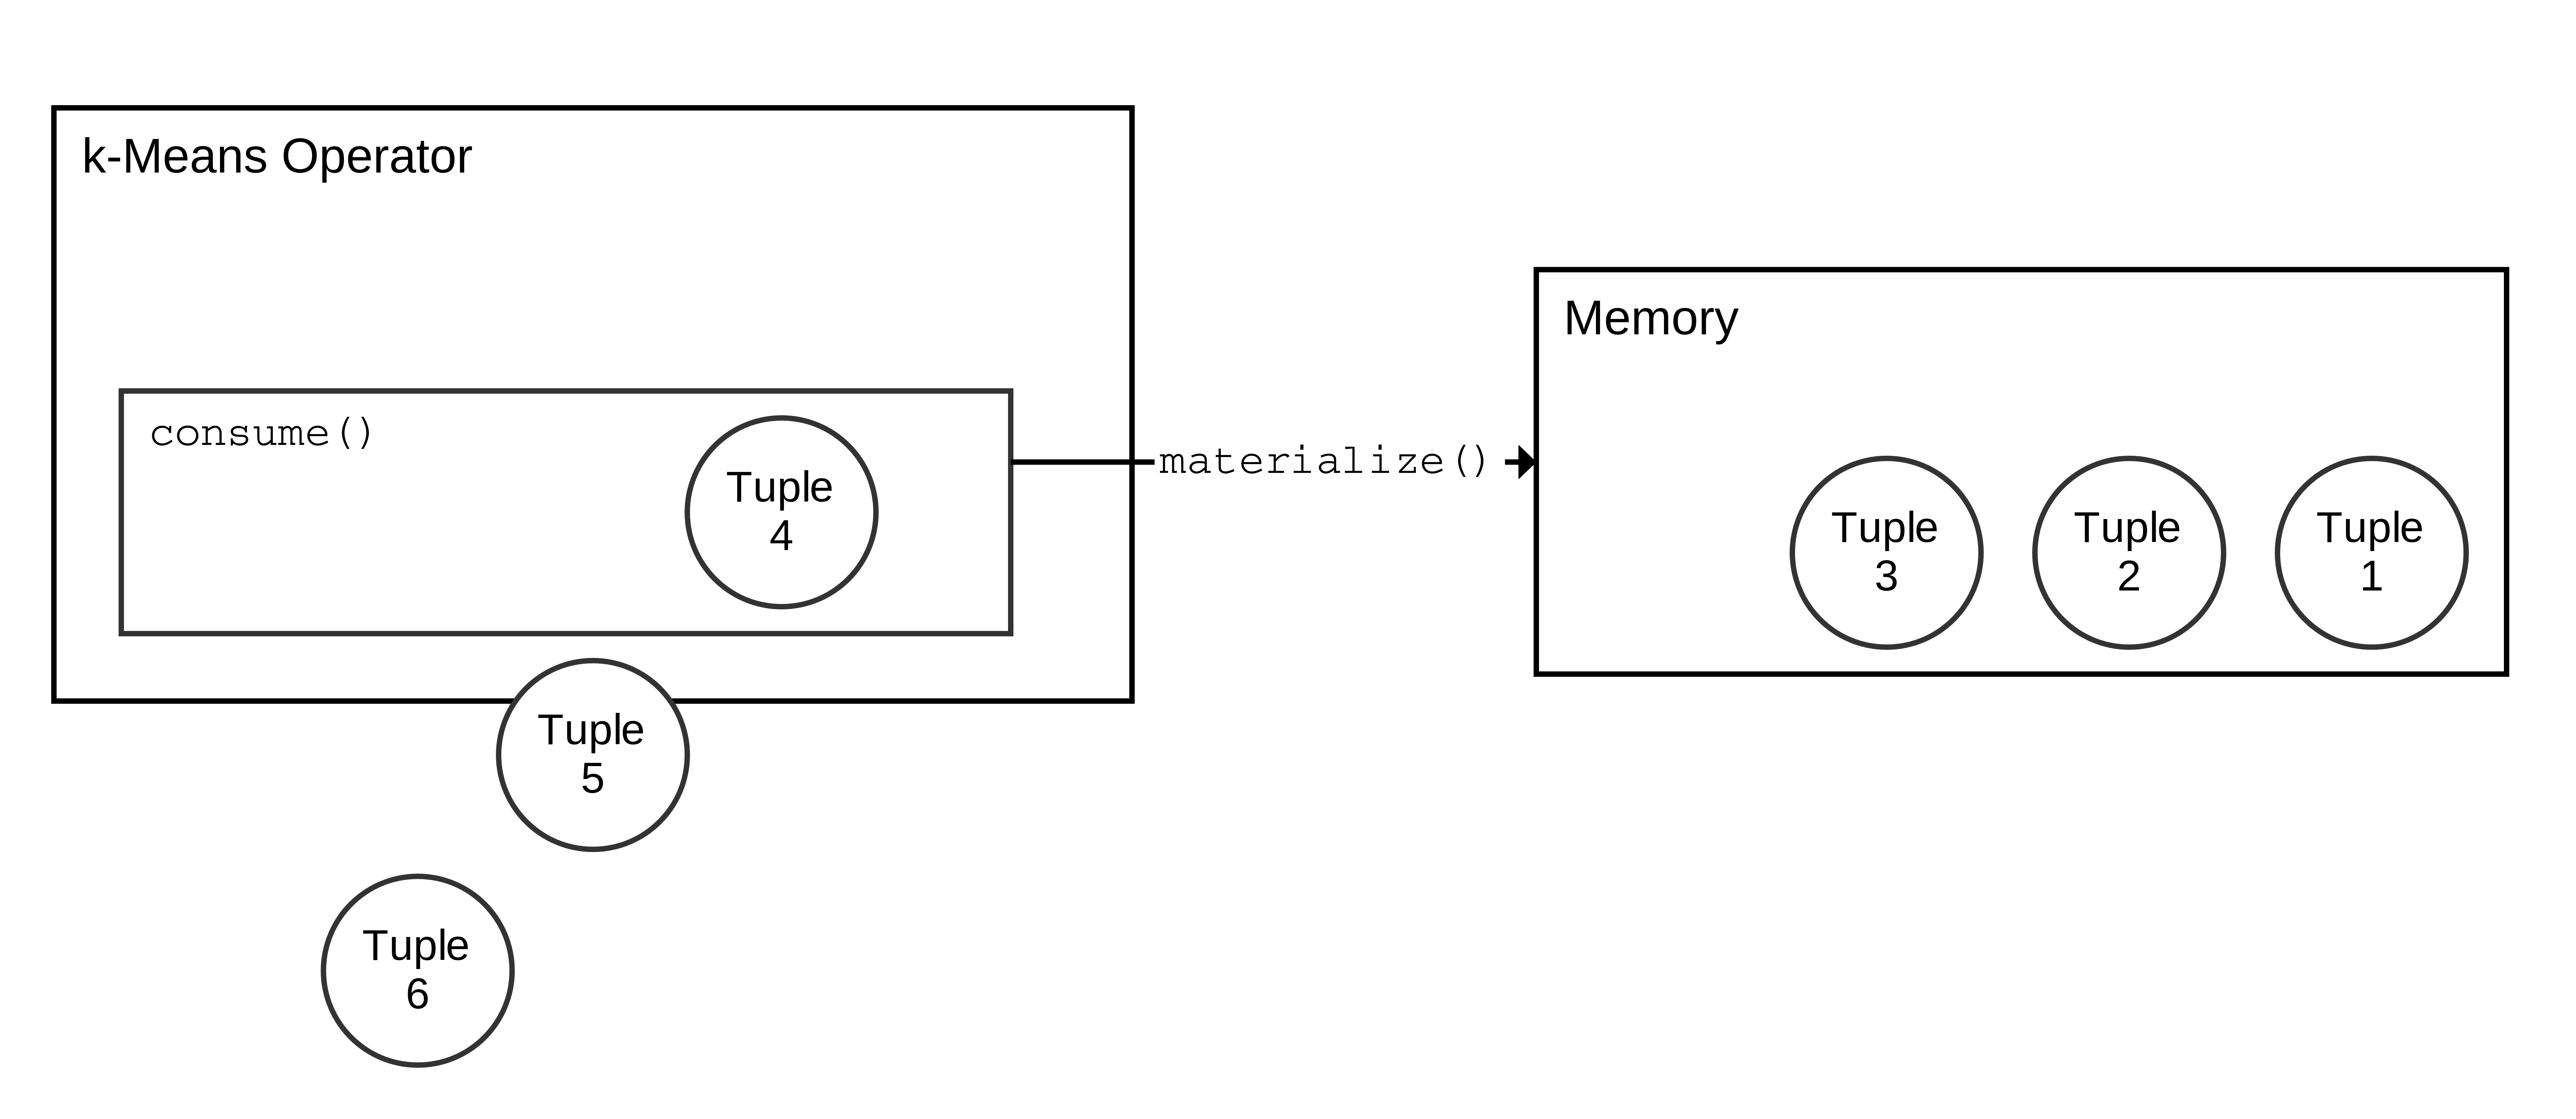
\includegraphics[scale=0.05]{figures/mat1_font2}
  }
  \caption[Data Materialization of Incoming Tuples]{Data Materialization of Incoming Tuples.}
  \label{fig:mat1}
\end{figure}

This is implemented by using a combination of LLVM and C++ code. In HyPer, LLVM code resides in the \texttt{compile time system (cts)} while C++ resides in the \texttt{runtime system (rts)}. Since the \texttt{compile time system} is the entry point of an operator, the \texttt{consume} function is called and generates code for each tuple. This generated code is materializing the incoming tuples. A pointer to the materialized chunk of memory is then stored in a C++ vector in the \texttt{runtime system}.~\autoref{fig:mat2} depicts this process: Each tuple is materialized into memory by the \texttt{cts} and can be referenced by a pointer stored in a vector in the \texttt{rts}. This vector can later be used to loop through the entire data set: First by looping through the vector in the~\texttt{rts}, getting the pointer to the memory location, which can then be used to load the tuple from memory into the CPU registers in the \texttt{cts}. 


\begin{figure}[htsb]
  \centerline{
  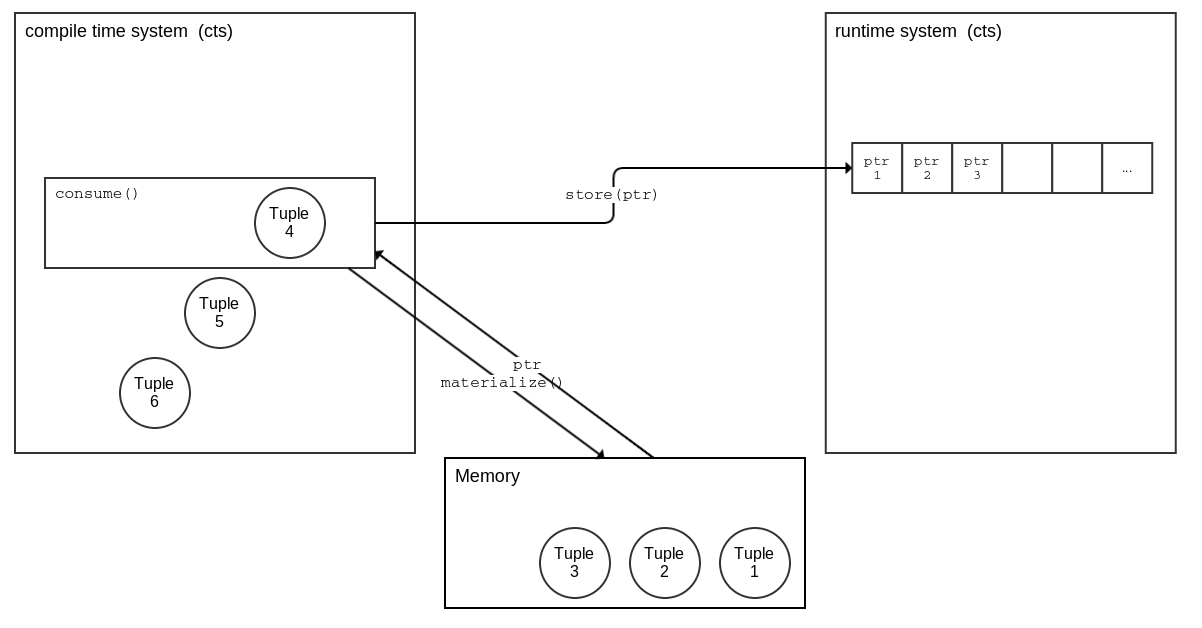
\includegraphics[scale=0.37]{figures/mat2_font3}
  }
  \caption[Data Materialization using the Runtime and Compile Time System]{Data Materialization using the Runtime and Compile Time System.}
  \label{fig:mat2}
\end{figure}

For k-Means it is not enough to store only the data tuples. We also need to reserve memory space for the centers. We do this by materializing the first \texttt{k} tuples of the data set two times: Once as storage for data tuples and once as storage for center tuples. Therefore we have two vectors in the \texttt{runtime system}: One for data tuples of length \texttt{n}, and one for centers of length \texttt{k}. This data materialization for k-Means is depicted in ~\autoref{fig:mat3}.
\\ 
At this point of the process, all data tuples and centers are materialized and an additional field has been added to all of them: A cluster identifier of type integer. For the center tuples, this field stores the center identifier, which goes from 0 to $k - 1$. For data tuples, this field specifies to which center and therefore to which cluster a data tuple belongs to. Initially, all data tuples are assigned to the center with identifier 0. 
\\
Another difference is the cast of data types between data and center tuples. While the data types of data tuples are specified by the table schema, the data types of the center tuples are determined differently since the center is the mean of all the data tuples assigned to that center. Therefore, an integer data value is stored as a numeric data type as center value. Numeric is an exact-value data type for integer and decimal types, and therefore able to store the mean of integer data tuple values. For each data type there exists a rule to cast the respective type from data to center tuple.



\begin{figure}[htsb]
  \centerline{
  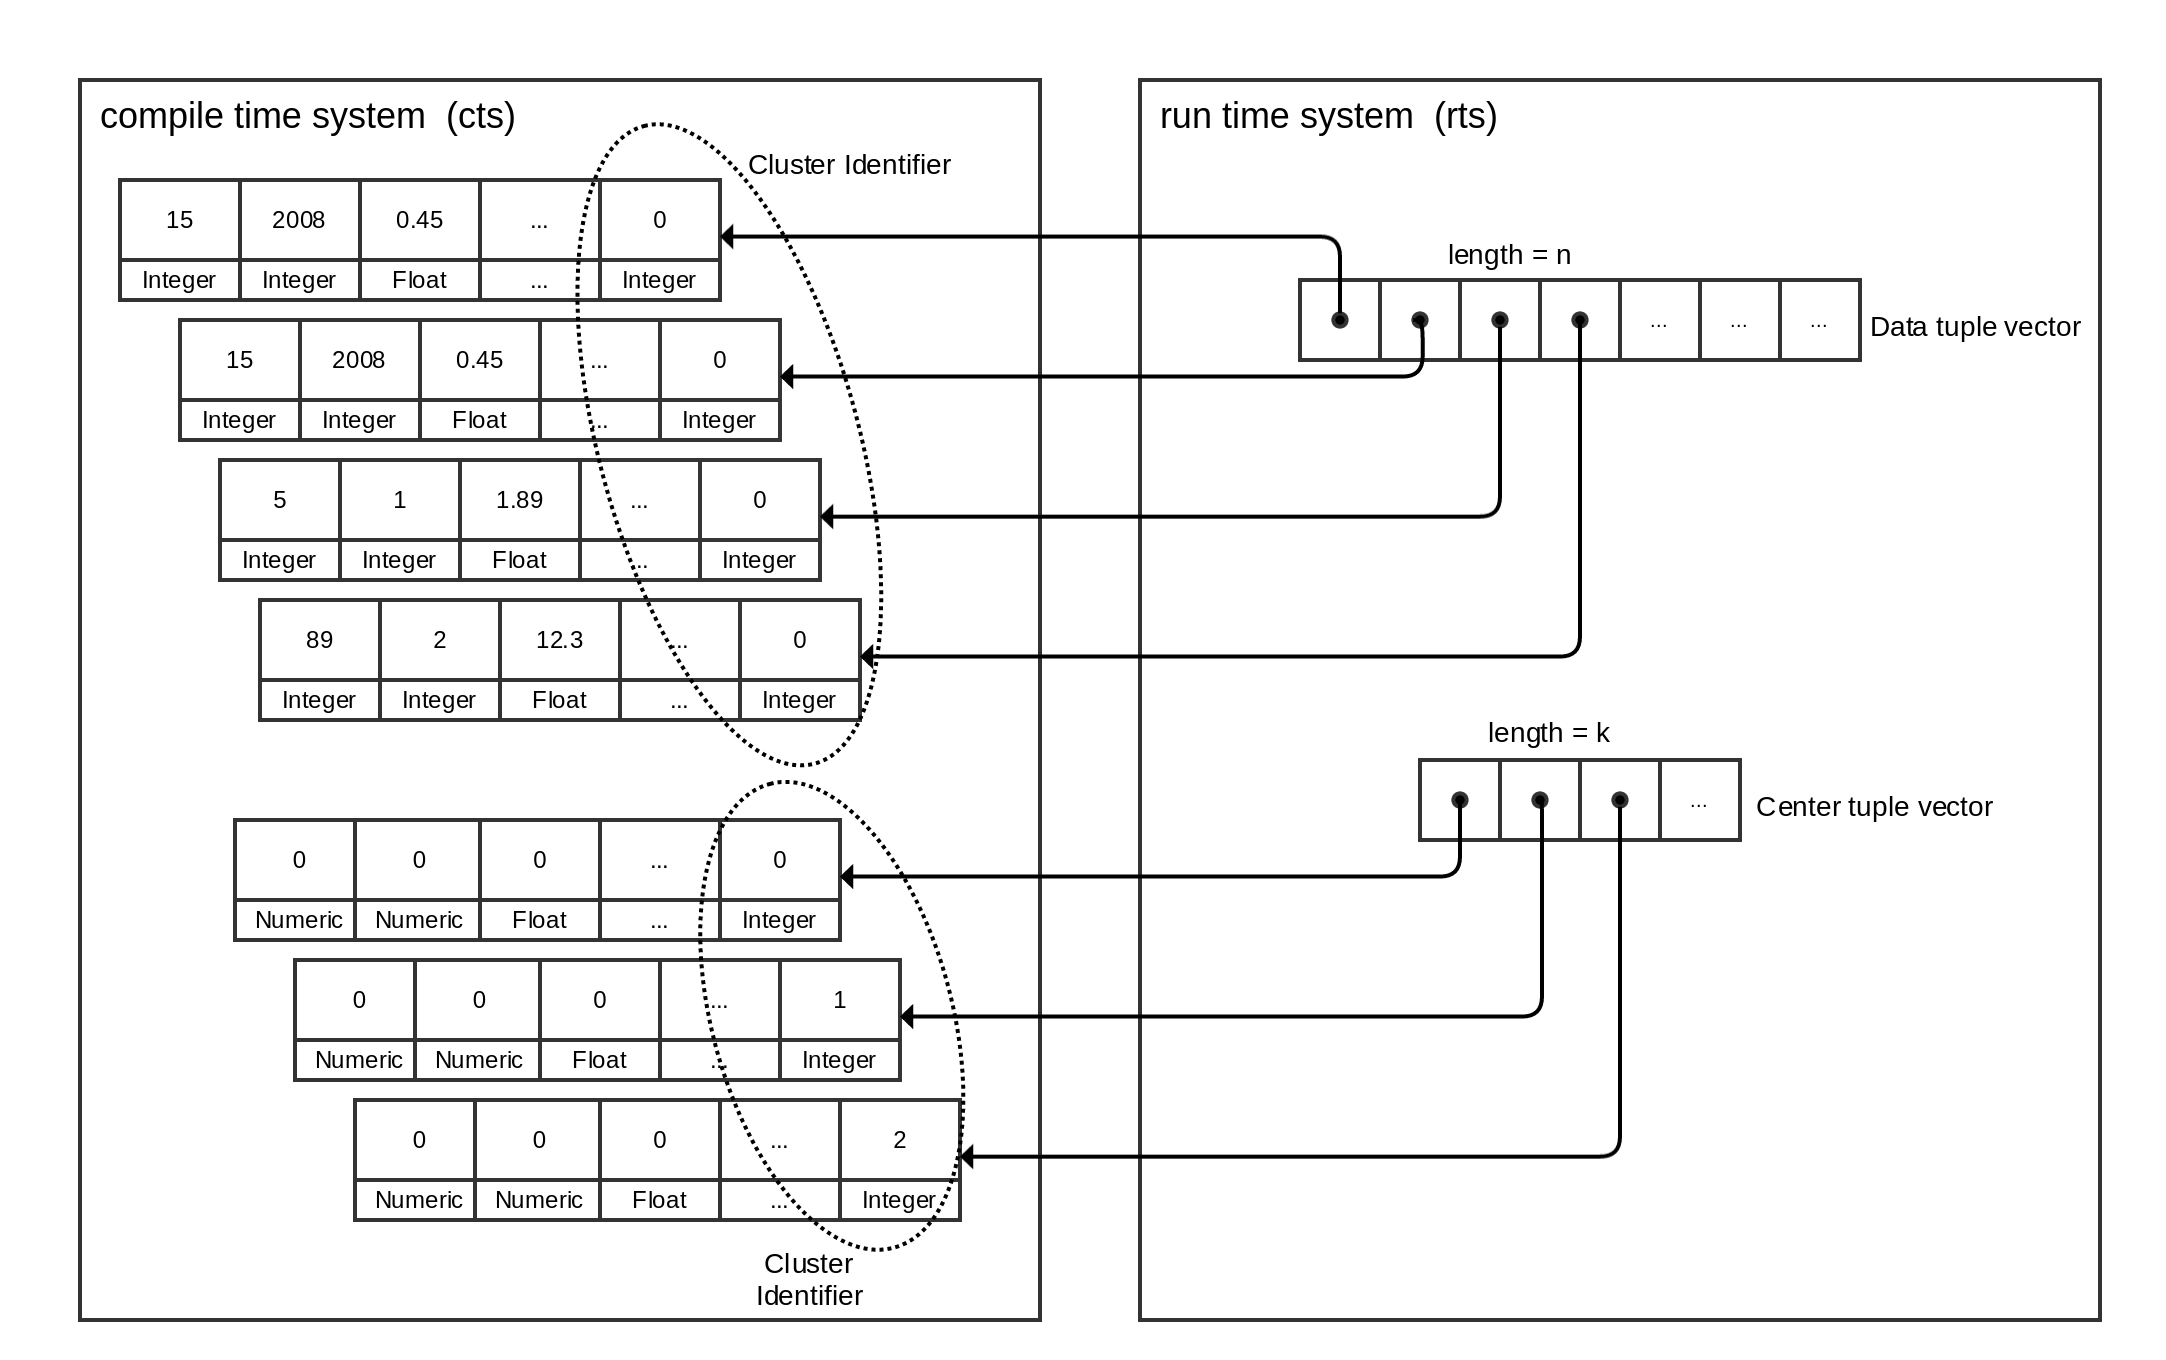
\includegraphics[scale=0.215]{figures/mat3_font2}}
  \caption[The k-Means Data Materialization in Detail]{The k-Means Data Materialization in Detail.}
  \label{fig:mat3}
\end{figure}


\section{Serial Implementation}\label{section:serial_implementation}

After acquiring a basic understanding of HyPer’s operator model, in particular about the interaction of dynamically generated LLVM code and pre-compiled C++ code, we can discuss the actual implementation of a serial k-Means algorithm. The most interesting part of implementing a data mining operator like k-Means in HyPer is the decision of the design of the algorithm, i.e. which parts of the code should reside in the \texttt{compile time system} and which parts in the \texttt{runtime system}. 
\\
This question is not trivial because there are no strict rules and several possibilities. For example, a dynamic generation of code works best for comparing tuples with each other as in the sort operator, or the computation of a distance in the k-Means operator. This code has to handle different data types depending on the table schema and therefore generated code is preferable. For other parts, like the implementation of a sort function or the combination of loops in k-Means, it is not so obvious where to put the code.
\\
In this work we present two different ways of implementing a serial k-Means operator in HyPer, first by implementing the algorithm in C++ with only a few generated LLVM functions, e.g. to compute the distance. Then, a system is presented implementing k-Means almost entirely in LLVM. Only small parts, like initializing the random centers are implemented in C++. This implementation benefits of generated, compact code and we expect performance gains over the C++ driven implementation.


\subsection{A C++ driven Implementation}

As first implementation approach we present a C++ driven version. The term C++ driven is maybe misleading, since all operators start their main computation after invoking their \texttt{consume} function, which is an LLVM generated function. Even though the operator starts working in the \texttt{compile time system}, in this implementation, \texttt{cts} calls the k-Means operator of the \texttt{runtime system} and gives the full control to the C++ code, until the k-Means algorithm terminates. 

~\autoref{fig:cpp_driven} shows this interaction in a sequence diagram: The algorithm is invoked in the \texttt{compile time system} and calls the k-Means function of the \texttt{runtime system}. The entire execution stays now in the \texttt{runtime system}, with calls back to the~\texttt{cts} from time to time, but immediately returns to the~\texttt{rts} once a function call terminates. 
\\
At first, the centers are selected. Let’s assume we are using a random initialization strategy. \texttt{K} times, a random pointer of the data vector is selected, and its values are copied to the corresponding center tuple. Therefore, the \texttt{centerPtr} and the randomly selected \texttt{dataPtr} are parameters of a generated \texttt{setCenter} function. This function loads both tuples from memory using its corresponding pointers. Next, the data values are casted if necessary, since we have different data types among center tuples and data tuples as described in the previous section, and then copied to the center tuple. Afterwards, the center tuple is written back to memory. This process is repeated until all $k$ centers are determined.

\begin{figure}[htsb]
  \centering
  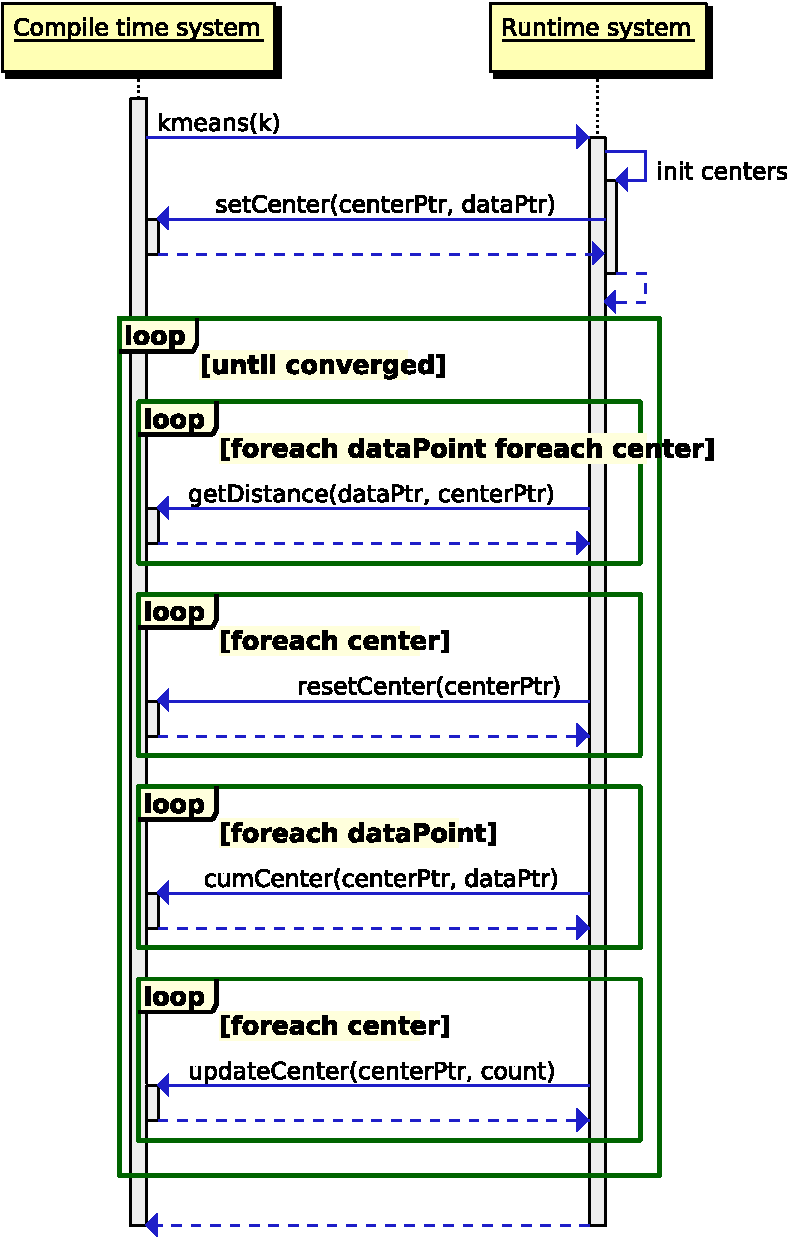
\includegraphics[scale=0.55]{figures/cpp_driven}
  \caption[The k-Means Algorithm - C++ driven]{The k-Means Algorithm - C++ driven.}
  \label{fig:cpp_driven}
\end{figure}

After selecting the initial set of centers, the \texttt{runtime system} starts its outer loop, running until k-Means converges. In the outer loop, the \texttt{runtime system} calls the \texttt{compile time system} to compute the distances between all data points and center points to find the closest center for each data tuple. Therefore, \texttt{getDistance} is invoked for each \texttt{dataPtr} - \texttt{centerPtr} combination. The closest center for each data point is then stored in an \texttt{unordered\_map} in C++ for efficient lookup. 
\\
After finding the closest center for each data tuple, the centers have to be updated. Since the materialization of centers is done in LLVM code, the \texttt{runtime system} has to call the \texttt{compile time system} again, in fact several times: First, a \texttt{resetCenter} function is called for all center pointers to set the center values of the center tuples to zero. Then, the new mean can be computed. 
\\
The computation of the mean is done in two steps. First, the data points are accumulated for each center, and then divided by the number of data points belonging to each center. This simple mean computation leads to several \texttt{compile time system} calls for our algorithm. For each data point, its values are added to the center tuple it belongs to. Therefore, the \texttt{cumCenter} function is called, adding the values of the data point to the center point and also updating the cluster identifier of the data tuple. The \texttt{runtime system} keeps track of how many tuples are added to each center. When finished, each center is called again to compute the actual mean of the center dividing by the count of data tuples assigned to the center using the \texttt{updateCenter} function. This concludes the first iteration of the algorithm. The next iteration starts then again with the computation of the closest center for the data points. This process continues until the algorithm converges.
\\
Using this implementation approach the main control of the algorithm remains in the \texttt{runtime system}. However, this kind of implementation leads to many calls between the \texttt{compile time} and the \texttt{runtime system}, in total $(n+2) \cdot k + n$ calls per iteration, as ~\autoref{tab:llvm_calls} shows. The next section presents an implementation that prevents the algorithm from too many calls between the two systems, which might affect the performance of the operator in a beneficial way.




\begin{table}[htsb]
  \caption[LLVM number of calls]{Generated Function Calls per Iteration.}\label{tab:llvm_calls}
  \centering
  \begin{tabular}{l l}
    \toprule
      Generated Function & Calls per Iteration \\
    \midrule
      \texttt{getDistance} & $k \cdot n$ \\
      \texttt{resetCenter} & $k$ \\
      \texttt{cumCenter} & $n$ \\
      \texttt{updateCenter} & $k$ \\
    \bottomrule
      Total & $k \cdot n + k + n + k = (n + 2) \cdot k + n$ \\
  \end{tabular}
\end{table}


\subsection{An LLVM driven Implementation}

As already stated, LLVM code generation encourages the interaction between LLVM and C++ code which is exploited a lot in the C++ driven implementation of k-Means: The algorithm is implemented in C++ and benefits from high-level data structures such as \texttt{unordered\_maps} and the convenience of the C++ syntax, allowing a quick implementation. 
\\
However, the approach presented in the previous section leads to many calls between the \texttt{compile time} and the \texttt{runtime system}, as shown in ~\autoref{tab:llvm_calls}, which could possibly affect the performance of the operator. Therefore, a second approach has been explored, implementing the k-Means algorithm almost entirely in LLVM code. Only the random initialization of the center points remains in C++. When thinking about such an implementation, we have to be aware that we cannot use C++ high-level data structures anymore, but have to work with what LLVM gives us.


\begin{figure}[htsb]
  \centerline{
    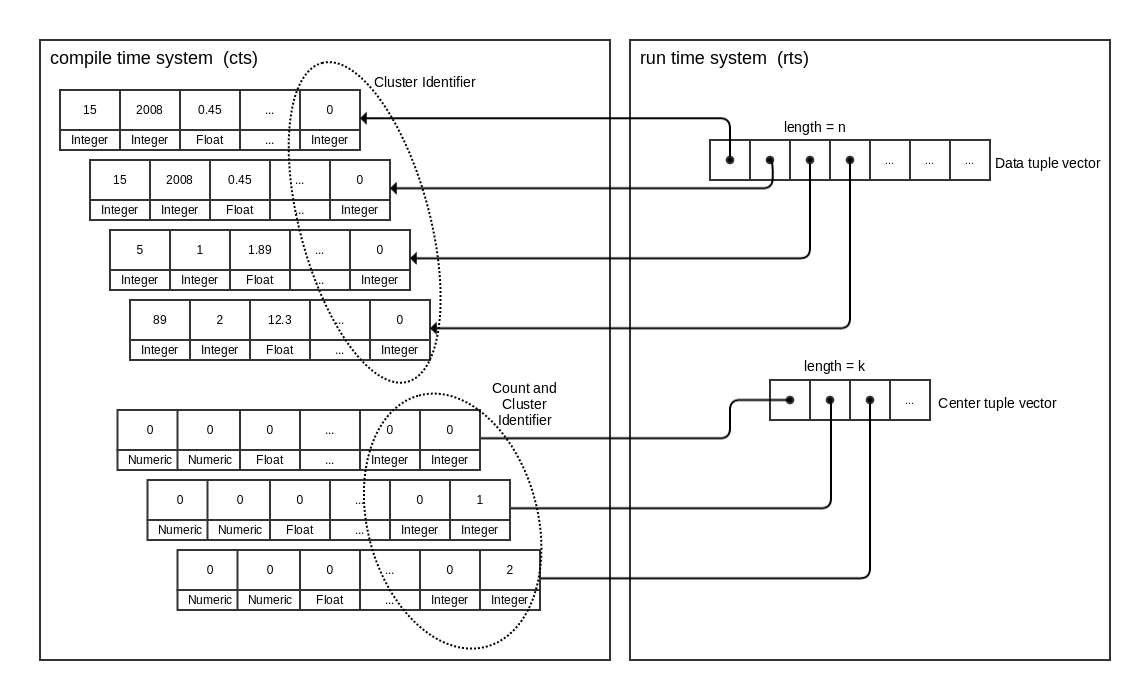
\includegraphics[scale=0.4]{figures/mat4_font}
  }
  \caption[The k-Means Data Materialization - LLVM Implementation]{The k-Means Data Materialization - LLVM Implementation.}
  \label{fig:mat4}
\end{figure}

The only data structure we have used so far in LLVM was a structure to materialize the data and center tuples. In order to keep things simple, we exploit this data structure even further to use it with the LLVM k-Means implementation, without using any other data structures in addition.
So the question is: How do we extend the existing data structure of the \texttt{compile time system} to emulate the C++ code we want to omit? This can be done by extending the center data structure when materializing the centers in the \texttt{consume} function. As ~\autoref{fig:mat4} shows, an additional field has been added to the center tuple to keep track of the count, determining how many data points are close to this center. With this small modification we can implement our algorithm in LLVM with the use of only one data structure.
\\
The LLVM driven algorithm is depicted in a sequence diagram in ~\autoref{fig:llvm_driven} and shows the indirection of the calls compared to the sequence diagram of the C++ driven approach in ~\autoref{fig:cpp_driven}: This time, the LLVM code executes the algorithm, calling C++ code from time to time. There are also no loops around the calls between the LLVM and C++ code, therefore the number of calls is very low. 
\\
As in the previous implementation, the algorithm starts with selecting the random centers. This process does not change, but afterwards the control of the algorithm goes back to the~\texttt{compile time system}. The only information the~\texttt{compile time system} requires from the~\texttt{runtime system} is the first pointer and the last pointer of the data vector and of the center vector, respectively. Then, the~\texttt{compile time system} is ready to execute the k-Means algorithm without any further interaction with the~\texttt{runtime system}. 
\\
Next, the minimum distances are computed between center and data tuples. The distance function was already implemented in LLVM code for the C++ driven approach and the code can be reused, only the loops around the \texttt{getDistance} function have to be implemented in LLVM. 
\\
The next step is to update the center tuples. The functionality of the \texttt{resetCenter} function can be kept the same, as well as the \texttt{cumCenter} function. Again, the loops around the functions are now implemented in generated LLVM code. When computing the mean of a center, we have to keep track of the count. For that purpose we are using the additional field of each center tuple created on data materialization. Whenever we are adding data tuples to the corresponding center, we increment the count. When invoking the \texttt{updateCenter} function, this count is used to compute the mean using a division. 



\begin{figure}[htsb]
  \centering
  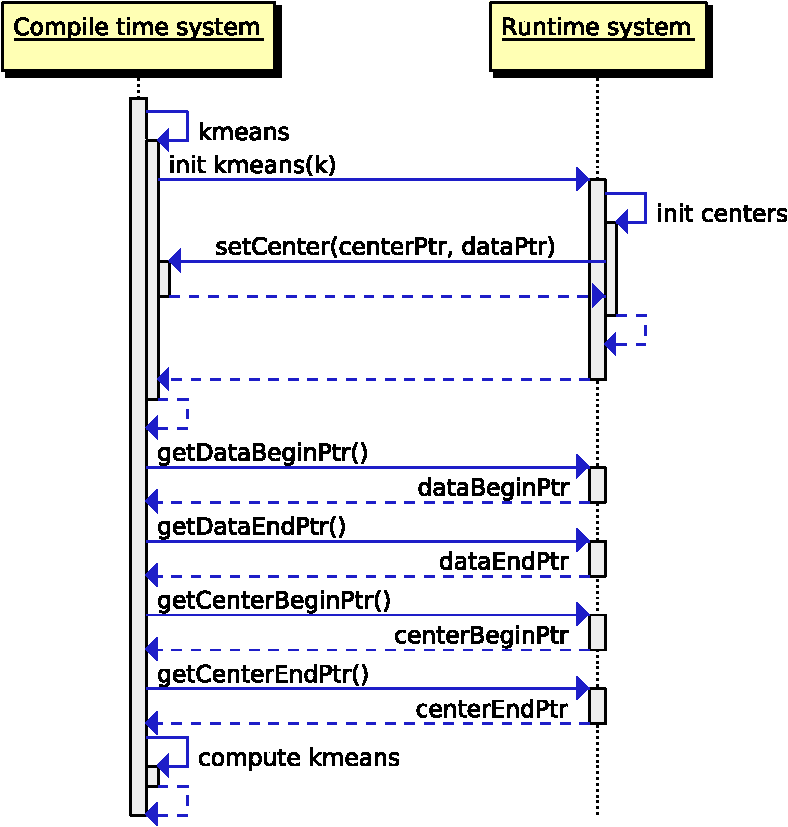
\includegraphics[scale=0.55]{figures/llvm_driven}
  \caption[The k-Means Algorithm - LLVM driven]{The k-Means Algorithm - LLVM driven.}
  \label{fig:llvm_driven}
\end{figure}



Even though the difference between the two presented approaches does not seem to be huge since the overall programming concept remains the same, the difference in the code is significant. In particular using LLVM over high-level C++ constructs adds an overhead in the number of code lines. Therefore, the LLVM code in the second approach is harder to understand and to maintain. On the other hand, we are shrinking the number of calls between the C++ and LLVM system from $(n + 2) \cdot k + n$ down to 4. This leads to performance improvements as we see in Chapter~\ref{chapter:evaluation}, where the LLVM driven approach shows better results for all carried out experiments.


\subsection{Initialization Strategy}\label{sub:init}

In the so far discussed implementation details of the k-Means algorithm we assumed to use a simple random initialization strategy. Such a strategy can be implemented in the~\texttt{runtime system}, since only C++ code is used for finding a random subset of length \texttt{k} of the data tuples, which can be implemented using the Fisher-Yates shuffle algorithm~\parencite{fisheryates}. 
\\
However, in Section~\ref{section:kmeans_init} we figured out that one of the most popular variations of k-Means is k-Means++. The k-Means++ algorithm uses an extended initialization strategy by choosing data points as center point with higher probability the further away they are from the already chosen set of center points. Often, this leads to improvements in both speed and quality of the clustering.
\\
For implementation this means that we have to compute the distance from the chosen center points to the data points in the initialization phase too. This can be done very conveniently for the C++ version, as the \texttt{getDistance} function is implemented already. Therefore, the main initialization routine can be written in C++, only the \texttt{getDistance} function is used as generated function.
\\
For the LLVM version, we still keep the center initialization in the \texttt{runtime system} to benefit of high-level C++ program structures. To realize the k-Means++ algorithm, we have to add an explicitly generated \texttt{getDistance} function to the LLVM code: Even though the LLVM version computes the distance as well, there is no generated function anymore, since the distance generation is part of the generated program. Once we have added this function, k-Means++ can be implemented the same way as in the C++ driven approach.

\section{Parallel k-Means}\label{section:parallel_implementation}

After presenting two single-threaded implementations of the k-Means algorithm, in this section we show an approach to implement k-Means in HyPer in a parallel way to make use of all cores. Keeping in mind that HyPer is a high-performance database system written in C++, it makes already excessive use of multi-threaded programs, therefore it is only logical to add a parallel version of k-Means too. In the following we use the serial C++ version and modify it to allow parallelism. The C++ version is used over the LLVM version due to higher maintainability, readability and the limited time of this work.
\\
The main bottleneck of the serial implementation is to compute the closest center for each data point: The algorithm has to calculate the distance to each center point which has to be performed in each iteration. This means $k \cdot n$ independent distance computations, which can benefit a lot from parallelism and a computation in independent threads.
\\
When executing a HyPer operator in parallel, the~\texttt{consume} function is called for chunks of input tuples instead of the entire data set. Consider a system with four threads as shown in~\autoref{fig:parallel}: Each thread consumes one fourth of the data set and materializes the input tuples. Also in the~\texttt{runtime system}, there are now vectors for each thread, storing the pointers to the input tuples. 


\begin{figure}[htsb]
  \centerline{
    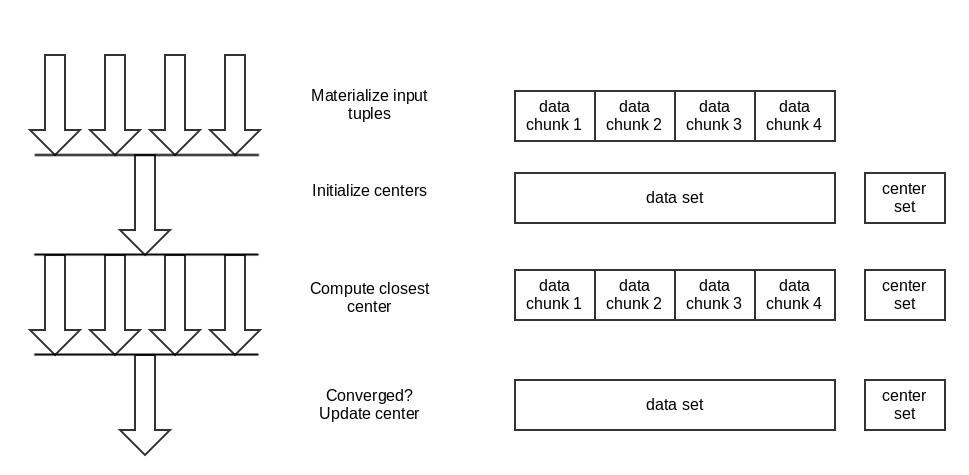
\includegraphics[scale=0.4]{figures/parallel_font}
  }
  \caption[The k-Means Algorithm as Parallel Operator]{The k-Means Algorithm as Parallel Operator.}
  \label{fig:parallel}
\end{figure}

After consuming the data the k-Means algorithm continues with choosing the initial center set. For that, we have to break with the parallelism: For a random initialization of the clusters, center tuples are selected from the entire data set randomly. This is even more important for the k-Means++ initialization strategy computing centers regarding a distance function. While we could select random data points for the center just from one data chunk, this is not possible anymore for the advanced logic of the k-Means++ initialization strategy. Therefore, we create a global vector storing pointers to all materialization tuples. Now we can select the global center points using one of our initialization strategies and continue the parallel program sequence afterwards.
\\
After this serial initialization we can continue the parallel execution of the algorithm and compute the distance from each data point to each center point. This expensive computation can be done independently in each data chunk on a separate thread and benefits from the potentials of parallelism. Ideally, this leads to a running time advantage of one fourth of the serial execution, however, due to the overhead of process creation and management we will not be quite able to attain such high improvements, as the experiments in Chapter~\ref{chapter:evaluation} show.
\\
After this parallel computation, we jump back to a serial execution mode and check for each thread if the program has converged. Only if all threads have converged, we can terminate the algorithm and output the result of the clustering. Otherwise, we update the center points by the newly assigned data points. In the first version of this parallel implementation, this step is done in serial as already presented in Section~\ref{section:serial_implementation}. However, here is potential for parallelizing the program even more, which is a goal for future implementations as we see in Chapter~\ref{chapter:conclusion}.
\\
In the evaluation chapter we compare the parallel k-Means algorithm with the two serial implementations. Even though only one part of the algorithm is parallelized and with the overhead of introducing the parallelism in mind, we expect huge performance gains since the parallelized code part contains many independent computations well-suited for multi-threaded execution.





